% Section 5.3.2: Machine Learning Model Development. New text is green (\newrevision).
% Input after 5.3.1 Planned Operating System and Runtime Environment, before 5.4.
\subsection{\newrevision{Machine Learning Model Development}}
\label{sec:ml_development}
\begingroup
\color{green!45!black}
\setlength{\emergencystretch}{2em}\sloppy
Two modelling approaches were developed offline on the same TreeVibes field recordings. Approach~A classifies short audio windows and was reduced to a small int8 model for the ESP32. Approach~B, tree-level multiple-instance learning (MIL), classifies a bag of consecutive recordings from one tree. This section records what was built and how it was trained. The experiments that led to each design choice, and their results, are reported in Section~\ref{sec:ml_results}.

\subsubsection{\newrevision{Common Data Source and Labels}}
\label{sec:ml_data}
Both approaches use the field recordings of the TreeVibes dataset \cite{rigakis2021}, version~1 of the Kaggle distribution. Recordings are 8~kHz WAV files of about 20~s, taken roughly every 5~minutes. Each folder holds the recordings of one monitored tree or deployment. The local inventory contains 58,797 WAV files: 4,154 field and 54,643 laboratory recordings. This is the same inventory used by the compression study in Section~\ref{sec:codec_results}.

Labels are assigned per folder. The dataset's AUDIO field, a listener's judgment, is copied to every recording in that folder, while the VISUAL and CONFIRMATION fields record external inspection and trunk slicing. The labels are therefore weak borer annotations, not species-confirmed red palm weevil labels. Exploratory analysis showed that many recordings labelled infested contain no audible evidence of infestation, because larval activity is intermittent. The team accepted clean recordings from other tree species (orange, fig, apricot and forest trees) as negatives and treated all recordings as acoustically comparable. This is a working assumption: the clean trees also differ from the infested palms in site, weather and recorder. Laboratory recordings were counted but not used to train Approach~A, because their parent recordings could not be traced.

Figure~\ref{fig:ml_eda} compares ten consecutive recordings from a healthy tree with ten from an infested tree.

\begin{figure}[htbp]
\centering
\IfFileExists{figures/overview_healthy_vs_infested.pdf}{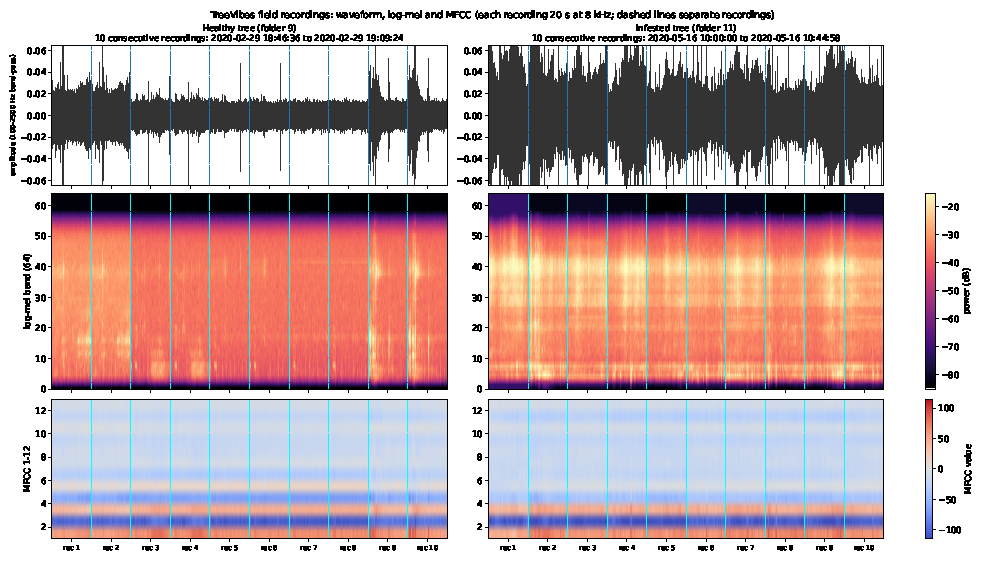
\includegraphics[width=\linewidth]{figures/overview_healthy_vs_infested.pdf}}{\fbox{\parbox{0.9\linewidth}{\centering\vspace{2cm}Figure file \texttt{overview\_healthy\_vs\_infested.pdf} not yet supplied.\vspace{2cm}}}}
\caption{\newrevision{Ten consecutive 20~s recordings from healthy folder~9 (29 February 2020) and infested folder~11 (16 May 2020): waveform, log-mel spectrogram and MFCC after a 100--2500~Hz band-pass filter, on the same colour scales. The two trees were recorded in different months with different recorders, so the visible differences are not due to infestation alone.}}
\label{fig:ml_eda}
\end{figure}

\subsubsection{\newrevision{Approach A: Clip-Level Classification and ESP32 Models}}
\label{sec:ml_dev_clip}

\paragraph{Overview.} Each window of audio receives a score, and the window scores are averaged into one score per recording. Three tracks were compared: an unrestricted track, a track limited to the 30~$\times$~13 MFCC input that suits feature transmission, and a track of int8 models for the ESP32. Four experiments, each motivated by the previous result, shaped the final design (Section~\ref{sec:ml_res_clip}).

\paragraph{Data and inputs.} After curation, 3,806 field recordings were kept and 348 were excluded because their source could not be traced. A locked split divided them into 1,476 training, 1,066 validation and 1,264 test recordings. Later cross-validation experiments used the 2,542 development recordings (1,567 infested and 975 clean, 30 folders). The ESP32 model input is a 1~s log-mel window of 59~$\times$~64 values: a 512-point Hann window, 128-sample hop, 64 HTK mel bands and a natural logarithm. Other inputs were the 30~$\times$~13 MFCC (40 mel filters, 13 coefficients), 10.24~s and 20.48~s log-mel segments, raw waveforms and summary statistics. On the ESP32, one decision is the mean of ten 1~s window scores. This pipeline applies no band-pass filter, no SNR gating and no signal squaring, and it is not the input of the compression study.

\paragraph{Evaluation protocol.} The locked split grouped recordings that share a device, site, tree, session, parent recording or identical audio, and was fixed by hashes before training. Later experiments used folder-grouped five-fold cross-validation and then leave-one-recorder-out cross-validation (seven folds). Thresholds were cross-fitted: each fold's threshold was chosen on the other folds. Selection was recall-oriented: recall at a validation false-positive rate (FPR) of at most 5\% in the first campaign, then rules based on F2, FPR~$\le$~10\% and 97\% training recall. For deployment, the threshold is calibrated on each device at the 90th percentile of scores from known-healthy trees. The final test split was never opened, because its lineage review was not completed.

\paragraph{Candidate models.} The first campaign trained 17 classical model families on five feature representations, and seven neural networks trained from scratch: a raw-waveform CNN, a log-mel CNN, a residual CNN, a CNN with a bidirectional GRU (CRNN), and an MLP, a CNN and a bidirectional GRU on MFCCs. Frozen pretrained embeddings (AST and Wav2Vec2) with logistic classifiers were also tested, as was a reproduction of the team's earlier \texttt{temporal\_w64} model. The ESP32 family uses only operations supported by TensorFlow Lite Micro (Table~\ref{tab:ml_esp32_models}). No CNN-LSTM or Mamba model was trained; the CRNN is the closest recurrent baseline.

\begin{table}[htbp]
\centering
\color{green!45!black}
\small
\caption{\newrevision{ESP32 int8 candidate architectures. Arena values are host lower bounds.}}
\label{tab:ml_esp32_models}
\begin{tabular}{llrr}
\toprule
Model & Layers & int8 size & Arena \\
\midrule
\texttt{stream1s\_w4} & conv 4/8/16, dense 8 & 7.8 KB & 18 KiB \\
\texttt{stream1s\_w8} & conv 8/16/32, dense 16 & 13.8 KB & 37 KiB \\
\texttt{stream1s\_w8\_d4} & conv 8/16/32/64, dense 16 & 35.3 KB & 37 KiB \\
\texttt{stream1s\_w16} & conv 16/32/64, dense 32 & 34.7 KB & 74 KiB \\
\texttt{stream1s\_ds} & conv 16, depthwise-separable 32/64 & 28.5 KB & 87 KiB \\
\texttt{strided10s\_w8} & 10.24~s input, stride-2 stem & 72.1 KB & 62 KiB \\
\texttt{dscnn10s\_res} & 10.24~s input, residual depthwise & 34.2 KB & 62 KiB \\
\bottomrule
\end{tabular}
\end{table}

\paragraph{Training setup.} Models were trained in PyTorch 2.5.1 with CUDA~12.1 on an NVIDIA RTX~2070 using mixed precision. The ESP32 models used AdamW (learning rate $2\times10^{-3}$, weight decay $10^{-2}$) with a one-cycle schedule for 20~epochs (1~s inputs) or 40~epochs (10~s inputs), and three random seeds. The loss was binary cross-entropy with extra weight on the infested class. SpecAugment, mixup and folder balancing were applied during training, and knowledge distillation from larger teachers was tried. Classical models used scikit-learn.

\paragraph{ESP32 conversion.} Each PyTorch model was rebuilt as an identical Keras graph, checked for matching outputs, and converted to a full-int8 TensorFlow Lite model with post-training quantization calibrated on training data (TensorFlow 2.18.1). A portable C99 front end computes the log-mel features as audio arrives, without storing whole recordings. The standalone benchmark firmware was built with ESP-IDF v5.3.6 and esp-tflite-micro 1.3.5, and Section~\ref{sec:esp32_deployment} describes the integrated firmware. The firmware runs one fold model and applies no alarm threshold.

\subsubsection{\newrevision{Approach B: Tree-Level Multiple-Instance Learning}}
\label{sec:ml_dev_mil}

\paragraph{Motivation and formulation.} Because labels describe a whole tree and many infested recordings are silent, Approach~B classifies a bag of $K$ consecutive recordings from one tree: $K=24$ (about 2~h) or $K=12$ (about 1~h). Each recording is encoded, a gated-attention layer weights the recordings, and a linear layer produces one probability per bag. Two encoders were used: a trainable CNN on 64~$\times$~626 log-mel spectrograms of 100--2500~Hz band-passed audio (257,666 parameters), and frozen AudioSet AST embeddings of 768 values per recording (99,266 trainable parameters). Larger heads, multi-head attention, a transformer, other pretrained encoders and six augmentations were also tested.

\paragraph{Grouping and splitting.} Folders that share identical recordings or lie within 5~m of each other were merged into one tree group. The development set had 2,477 recordings in 21 groups, of which 5 were healthy. Models were evaluated with ten tree-group folds, in which each tree group is scored by a model that never saw it, and with leave-one-recorder-out folds. Because half of the folds contain no healthy group, false alarms cannot be measured fold by fold; the scores from all folds were therefore combined before each metric was computed, instead of averaging per-fold metrics. Four groups (1,284 recordings) were sealed as a one-time holdout.

\paragraph{Training and selection.} Each step drew three healthy and three infested bags. Training used Adam (learning rate $3\times10^{-4}$, weight decay $10^{-4}$) with a cosine schedule for a fixed 30 epochs of 64 steps. The weights after the final epoch were used, with no early stopping and no choice of a best epoch, because choosing an epoch on the held-out trees would have made the results optimistic. A change was adopted only if three conditions held: its gain in tree-weighted AUC or balanced accuracy had a 95\% interval above zero in a paired tree bootstrap, the gain was larger than the difference between two baseline seeds, and the other metric did not get significantly worse. In the paired tree bootstrap, the tree groups were resampled with replacement 1,000 times, healthy and infested groups separately, and both models were scored on the same resampled trees each time. The alarm threshold was fixed at 0.5. Four experiments shaped the approach (Section~\ref{sec:ml_res_mil}).

\subsubsection{\newrevision{Final Model Selection}}
\label{sec:ml_selection}
The selected embedded model is \texttt{stream1s\_w8\_d4} from Approach~A, deployed as a single int8 model that scores 1~s windows, with per-device threshold calibration. It was chosen on five criteria, in order: behaviour on recorders not seen in training; a recall-oriented operating point after per-device calibration; fit within ESP32 flash and RAM using supported operations only; a successful build and run on the board with output matching the offline reference; and a single model rather than an ensemble. It has four convolution blocks (8, 16, 32 and 64 channels) with max-pooling, global average pooling, a 16-unit dense layer and a sigmoid output. Its input is one 59~$\times$~64 int8 log-mel window per second, and ten windows are averaged per 10~s decision. \texttt{stream1s\_w16} gave the best result without calibration, but it needs about twice the tensor arena, more than the 64~KiB the firmware reserves, and about 2.6 times the computation, and it did worse after per-device calibration. Approach~B was not selected: its best encoder, the frozen AST, cannot run on the ESP32 as built, and its alarm threshold did not transfer to new trees.

\paragraph{Code and data availability.} Approach~A's notebook, scripts, split hashes and firmware model are in the project simulation repository. Approach~B's scripts, configurations and fold definitions are stored with its 526 checkpoints on the training computer. Appendix~\ref{app:ml_log} lists all experiments.
\endgroup
